\documentclass[14pt]{beamer}

\usepackage{hyperref}

\newcommand{\cC}{{\mathcal C}}
\newcommand{\cE}{{\mathcal E}}
\newcommand{\cL}{{\mathcal L}}
\newcommand{\cW}{{\mathcal W}}
\newcommand{\cH}{{\mathcal H}}
\newcommand{\cT}{{\mathcal T}}
\newcommand{\cS}{\mathcal S}
\newcommand{\cO}{\mathcal O}
\newcommand{\cP}{\mathcal P}
\newcommand{\eps}{\varepsilon}
\newcommand{\BB}{\mathbb{B}}
\newcommand{\R}{\mathbb{R}}
\newcommand{\N}{\mathbb{N}}
\newcommand{\F}{\mathbb{F}}
\newcommand{\Z}{\mathbb{Z}}

\mode<presentation>
{
  \usetheme{Darmstadt}
  \setbeamercovered{transparent}
  % or whatever (possibly just delete it)
}


\usepackage[english]{babel}

\usepackage[latin1]{inputenc}

\usepackage{times}
\usepackage[T1]{fontenc}
\usepackage{graphicx}
\usepackage{graphics}

\title[Bikeshare]
{Capital Bikeshare Station and Ride Analysis\\
Eric Buras$^*$ and Hans Engler}


\begin{document}


\begin{frame}
  \titlepage
\end{frame}

\frame{
\frametitle{Bikeshare Station}
\begin{center}
\resizebox{3in}{!}{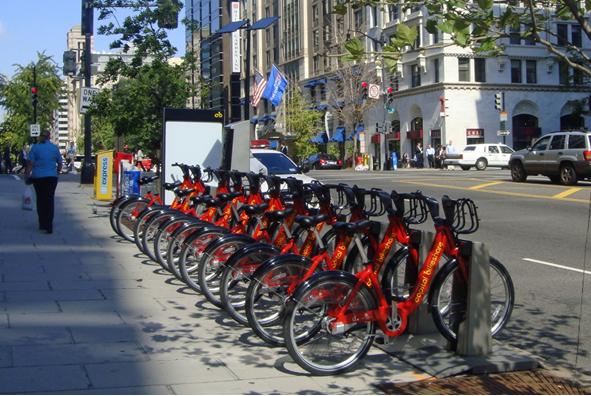
\includegraphics{bikes.png}} 
\end{center}
}

\frame{
\frametitle{The System}
\begin{itemize}
\item
Started in 2010. As of 4th quarter 2013 there are over 300 stations and ~750,000 rides/quarter
\item
Data made freely available with start and end date, time, and station, and rider type
\item
\texttt{0h 5m 41s, 6/30/2013 23:51, Florida Ave \& R St NW, 31503, 6/30/2013 23:56, 5th \& K St NW, 31600, W01380, Subscriber}
\item
Large Scale system concerns, other systems 
\end{itemize}
}

\frame{
\frametitle{Registered vs. Casual Riders}
\begin{center}
\resizebox{4in}{!}{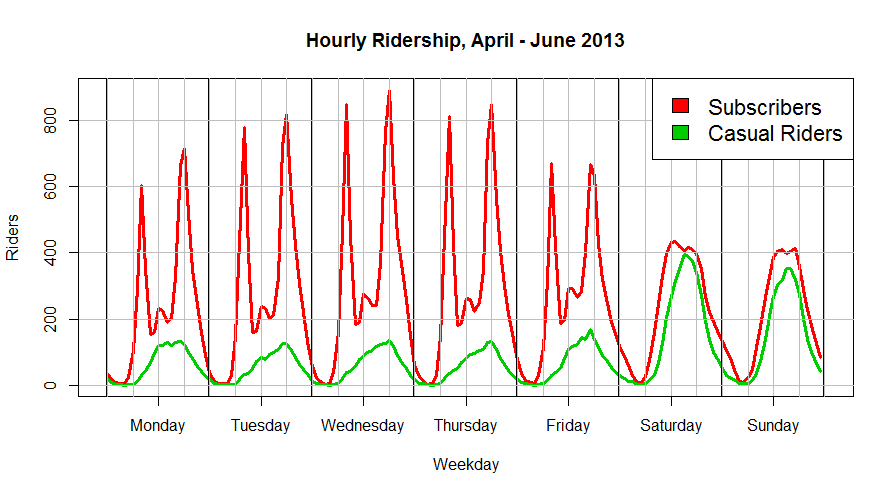
\includegraphics{ridership.png}} 
\end{center}
}

\frame{
\frametitle{Our Work}
\begin{itemize}
\item 
Applying Expectation-Maximization algorithm to the ride data for different models in R Statistical Software
\item 
Want to cluster ride data by a latent variable to analyze different variables (rider type, start/end station, time of day, start and end station pairs)
\item
Identify traffic flow, similar stations, ridership patterns
\item 
Following similar work done on Velib` system in Paris
\end{itemize}  
}

\frame{
\frametitle{Expectation Maximization - 1}
\begin{itemize}
\item
Given data $(x_i, z_i) \sim f(x,z;\lambda)$, where $\lambda$ is an unknown parameter vector
\item
Can estimate $\lambda$, using e.g. maximum likelihood
\item
\textbf{What if the $z_i$ are unobserved?}
\item
Try to estimate $\lambda$ from just the $x_i$ 
\item
Try to find expected values of the $z_i$ as well
\end{itemize}  
}

\frame{
\frametitle{Expectation Maximization - 2}
\begin{itemize}
\item
Iterative procedure (Expectation step alternating with maximization step) that is proven to converge
\item 
Expectation (E) step: Compute (update) the expected value of the unobserved $z_i$, given the data $x_i$ and the current value of $\lambda$
\item 
Maximization (M) step: Maximize the log likelihood function to compute $\lambda$, given the data and the current expected $z_i$ values
\end{itemize}  
}

\frame{
\frametitle{Model I: Clusters of Stations}
\begin{itemize}
\item
Station number $1 \le i \le  N \approx 230$, 
time $t \in \{0,\dots,23\}$ , day  
$d \in \{1, \dots,91\}$, cluster $\ell$ 
\item
$X_{itd}$ =  count of rides starting (or ending) at station $i$ at time $t$ on day $d$, \textbf{observed} 
\item
$Z_{i\ell} =1 $ iff station $i$ is in cluster $\ell$,  $Z_{i \ell} = 0$ otherwise, \textbf{not observed}
\end{itemize}  
}


\frame{
\frametitle{Model I Assumptions}
\begin{itemize}
\item
Conditioned on $Z_{i\ell} = 1$, assume $X_{itd} \sim 
\mathfrak{P}(\alpha_i \cdot \lambda_{\ell t})$ (Poisson)
\item
Suitable independence assumptions
\item
$\alpha_i$ = mean hourly count at station $i$
\item
$\lambda_{\ell t}$ = relative hourly intensities for cluster $\ell$    

\end{itemize}  
}

\frame{
\frametitle{EM Algorithm for This Case}
\begin{itemize}
\item
Only need to update the $\lambda_{\ell t}$ and the expected values for $Z_{i\ell}$. The $\alpha_i$ are computed only once. 
\item
E-Step: Calculate expected values of $Z_{i\ell}$ with Bayes Rule, using the data $X_{itd}$ and the current estimates of the $\lambda_{\ell t}$.
\item
M-Step: Maximum likelihood estimate of the $\lambda_{\ell t}$, using the data $X_{itd}$ and expected values of $Z_{i \ell}$ 
\end{itemize}  
}

\frame{
\frametitle{Algorithm Implementation and Outcome}
\begin{itemize}
\item
Simplify update equations to run in R quickly
\item 
Use matrix algebra and array manipulation
\item 
Implementation very efficient even on personal laptop
\item
Obtain $\lambda_{\ell t}$ (hourly intensities for each cluster)
\item
Obtain estimates for $Z_{i \ell}$ (cluster membership for each station)
\end{itemize}
}

\frame{
\frametitle{Results for Model I: Intensities}
\begin{center}
\resizebox{4in}{!}{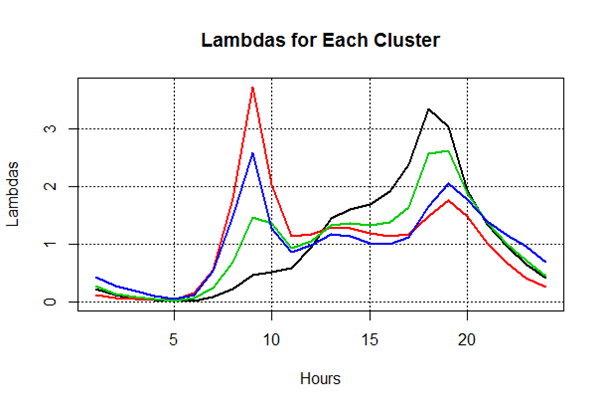
\includegraphics{lambdas1.png}} 
\end{center}
}

\frame{
\frametitle{Results for Model I: Clusters}
\begin{center}
\resizebox{4in}{!}{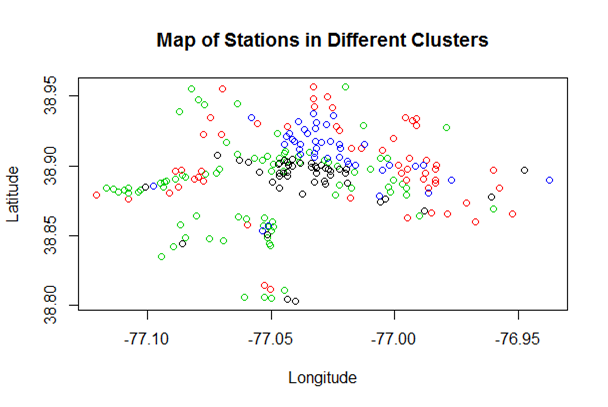
\includegraphics{clusters.png}} 
\end{center}
}

\frame{
\frametitle{Model II: Clusters of Station Pairs}
\begin{itemize}
\item
Start and end station $i, \, j$, 
time $t$, day 
$d$, cluster $\ell$ 
\item
$X_{ijtd}$ = count of rides from station $i$  to $j$ at time $t$ on day $d$ 
\item
$Z_{i j \ell} =1 $ iff station pair $(i,j)$ is in cluster $\ell$, $Z_{ij \ell} = 0$ otherwise 
\end{itemize}  
}

\frame{
\frametitle{Model II Assumptions}
\begin{itemize}
\item
Conditioned on $Z_{i j \ell} = 1$, assume $X_{i j td} \sim 
\mathfrak{P}(\alpha_{ij} \cdot \lambda_{\ell t})$ (Poisson)
\item
Suitable independence assumptions
\item
$\alpha_{ij}$ = mean hourly ride count from station $i$ to station $j$
\item
$\lambda_{\ell t}$ = relative hourly intensities for cluster $\ell$    
\end{itemize}  
}


\frame{
\frametitle{Model II: Clusters of Station Pairs}
\begin{itemize}
\item 
Clusters according to Station-Station pair ride count
\item
EM Algorithm applied to ride data with station pair scaling factor $\alpha_{ij}$ 
\item
There are many station pairs with few or no rides between them 
\item 
These station pairs cannot be assigned to a cluster (there is no estimated $Z_{ij \ell}$ that is close to 1) 
\end{itemize}  
}


\frame{
\frametitle{Results for Model II: Intensities}
\begin{center}
\resizebox{3in}{!}{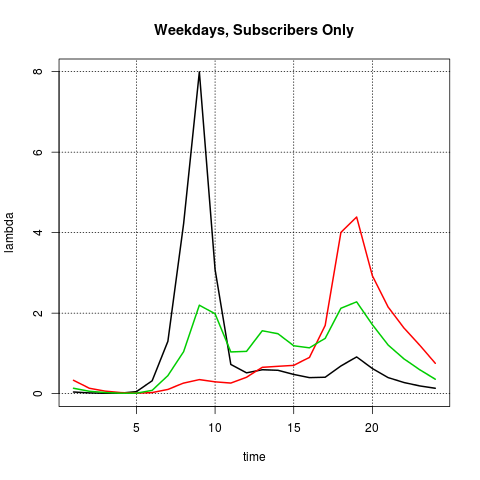
\includegraphics{lambdasm2.png}} 
\end{center}
}


\frame{
\frametitle{Union Station Outbound}
\begin{center}
\resizebox{2.7in}{!}{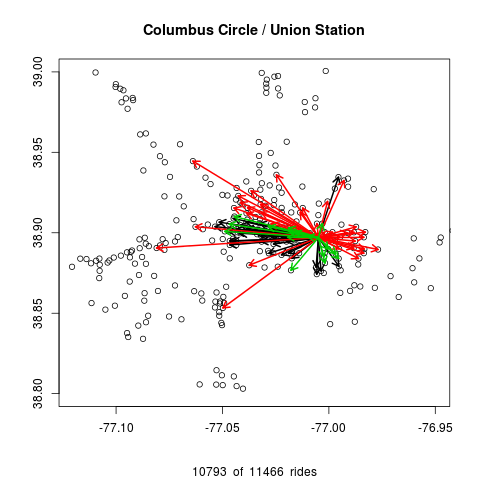
\includegraphics{31623out.png}} 
\end{center}
}


\frame{
\frametitle{Union Station Inbound}
\begin{center}
\resizebox{2.7in}{!}{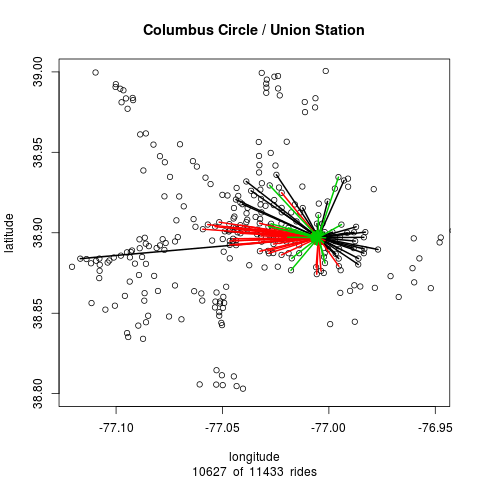
\includegraphics{31623in.png}} 
\end{center}
}


\frame{
\frametitle{$19^{th}$ and Penn NW Outbound}
\begin{center}
\resizebox{2.7in}{!}{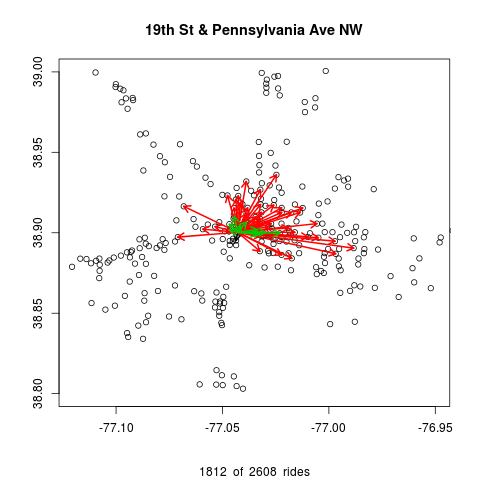
\includegraphics{31100out.png}} 
\end{center}
}


\frame{
\frametitle{$19^{th}$ and Penn NW  Inbound}
\begin{center}
\resizebox{2.7in}{!}{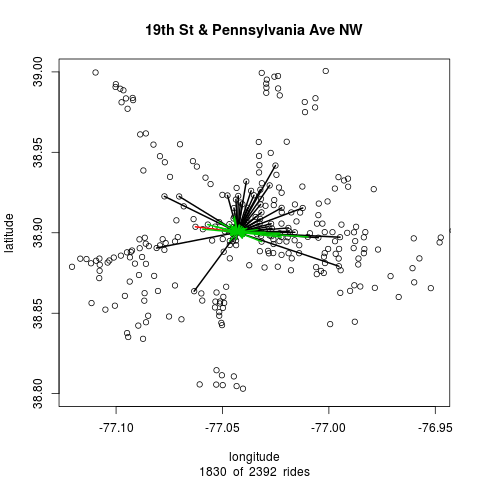
\includegraphics{31100in.png}} 
\end{center}
}

\frame{
\frametitle{Dupont Circle Outbound}
\begin{center}
\resizebox{2.7in}{!}{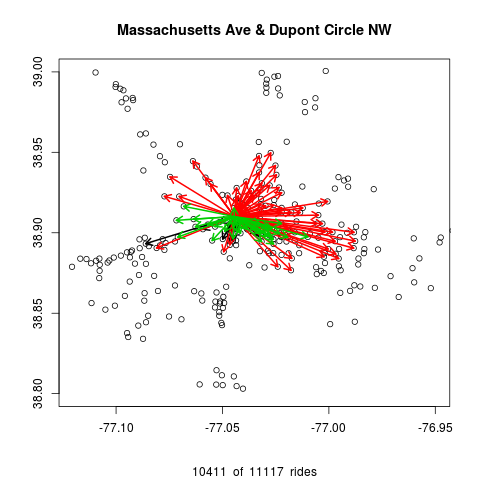
\includegraphics{31200out.png}} 
\end{center}
}


\frame{
\frametitle{Dupont Circle Inbound}
\begin{center}
\resizebox{2.7in}{!}{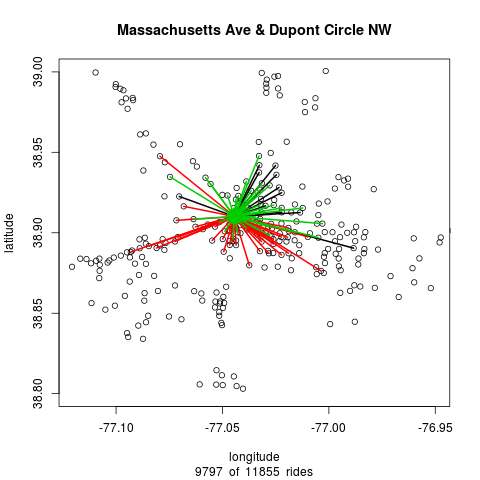
\includegraphics{31200in.png}} 
\end{center}
}


\frame{
\frametitle{$19^{th}$ and E NW Outbound}
\begin{center}
\resizebox{2.7in}{!}{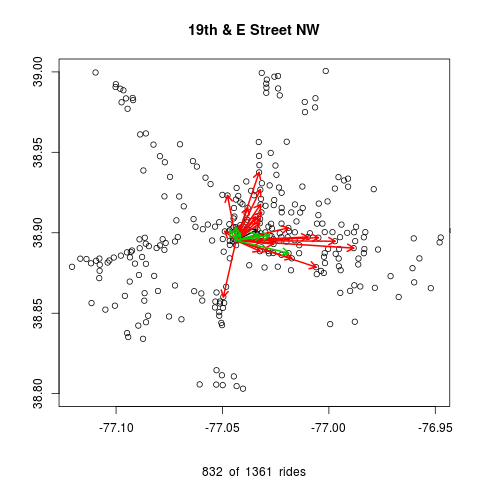
\includegraphics{31206out.png}} 
\end{center}
}


\frame{
\frametitle{$19^{th}$ and E NW  Inbound}
\begin{center}
\resizebox{2.7in}{!}{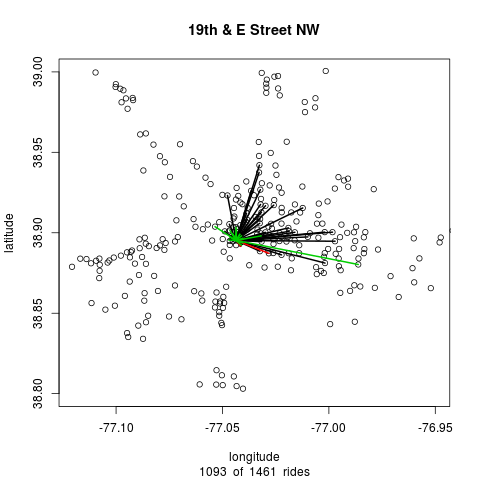
\includegraphics{31206in.png}} 
\end{center}
}



\frame{
\frametitle{Georgetown University Outbound}
\begin{center}
\resizebox{2.7in}{!}{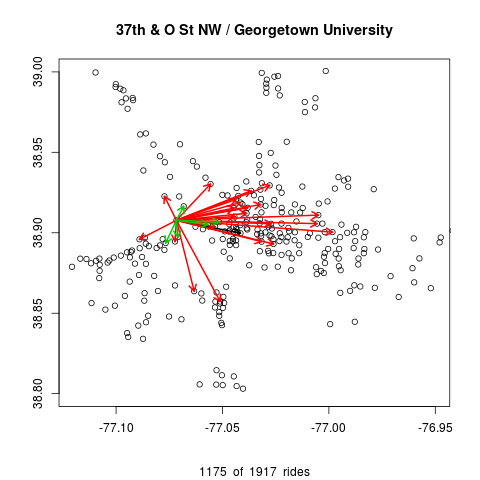
\includegraphics{31236out.png}} 
\end{center}
}


\frame{
\frametitle{Georgetown University Inbound}
\begin{center}
\resizebox{2.7in}{!}{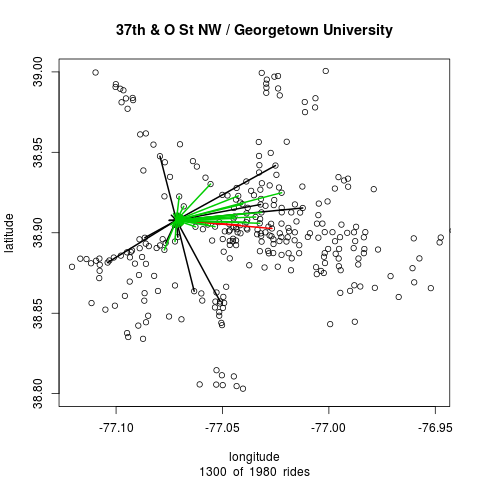
\includegraphics{31236in.png}} 
\end{center}
}

\frame{
\frametitle{Variability and Performance}
\begin{itemize}
\item
Variability comes from random initialization of $\lambda_{\ell t}$ before running EM 
\item
Model 1 has more rides per station than Model 2 has rides per station pair, so there is less variability between runs 
\item
More rides means that Model 1 converges much faster than Model 2
\item
Increasing the number of clusters too much makes results harder to interpret as clusters will be similar
\item
Decreasing the number of clusters too much leaves out information 
\end{itemize}  
}

\frame{
\frametitle{Conclusions}
\begin{itemize}
\item
This is a toolset to describe ridership flow. There is no mathematical result!
\item
Could be used to explore bikeshare systems in NYC, etc. and other systems that have established pickup/dropoff locations (uber/lyft?)
\item
Further Research: Exploring how the bikeshare system evolves:
\begin{itemize}
\item 
Ridership patterns emerge over time as users learn how to use the system better
\item
Seasonal patterns 
\item 
Rebalancing stations
\end{itemize}
\end{itemize}  
}

\end{document}

\frame{
\frametitle{}
\begin{itemize}
\item
\end{itemize}  
}

\frame{
\frametitle{}
\begin{itemize}
\item
\end{itemize}  
}

\frame{
\frametitle{}
\begin{itemize}
\item
\end{itemize}  
}

\frame{
\frametitle{}
\begin{itemize}
\item
\end{itemize}  
}

\frame{
\frametitle{}
\begin{itemize}
\item
\end{itemize}  
}


\end{document}



\frame{
\frametitle{Keeling Curve -- 2/4}
\begin{center}
\resizebox{2.1in}{!}{\includegraphics{figures/HawaiiSnow.png}} \\\vspace{2ex}
Mauna Loa and Mauna Kea
\end{center}
}

\frame{
\frametitle{Keeling Curve -- 3/4}
\begin{center}
\resizebox{3.3in}{!}{\includegraphics{figures/Mauna-wk1-2011.png}} \\\vspace{2ex}
Raw $CO_2$ Data from January 1-7, 2011
\end{center}
}


\frame{
\frametitle{Keeling Curve -- 4/4 }
\begin{center}
\resizebox{3.2in}{!}{\includegraphics{figures/MaunaLoaCO2.png}} \\\vspace{2ex}
Keeling Curve
\end{center}
}



\end{document}


